\documentclass[{../../master}]{subfiles}
\graphicspath{{../..}}  % 個別コンパイル時の画像パスを解決する

\begin{document}

\section{URDFモデリング用パッケージの作成}
\label{sec:create_urdf_package}

\subsection{ディレクトリ構成}

ここから実際にURDFモデリングを行っていきます.
まずは,URDFモデルを置くためのROSパッケージを作成します.
慣習的に,ロボットのURDFモデルは\textsf{*\_description}(*はロボットもしくはプロジェクトの名前)という名前のROSパッケージに配置します.
ADAMR2プロジェクトならば「\textsf{adamr2\_description}」という名前になります.
URDFモデリングを始める前にパッケージを作っておきましょう.
ビルド依存パッケージは無いので,パッケージ作成コマンドにオプションは必要ありません.

\begin{lstlisting}[language=sh, caption=Create a Package to put the URDF Model in]
catkin create pkg adamr2_description
\end{lstlisting}

パッケージが作成できたら,中にいくつかのディレクトリを作成します.
\textsf{adamr2\_description}パッケージのディレクトリ構成はコード\ref{code:package_directory_structure}のようにします.

\begin{lstlisting}[language=sh, caption=Directory Structure of adamr2\_description, label=code:package_directory_structure]
adamr2_description/
  ├ launch/
  ├ meshes/
  ├ rviz/
  ├ urdf/
  ├ package.xml
  └ CMakeLists.txt
\end{lstlisting}

\textsf{launch/}ディレクトリには,URDFモデルの可視化を行うためのlaunchファイルを置きます.
\textsf{meshes/}ディレクトリには,STL形式のロボットの3Dモデルを置きます.
\textsf{rviz/}ディレクトリには,URDFモデル可視化時の\textsf{rviz}の設定ファイルを置きます.
そして,\textsf{urdf/}ディレクトリにxacroファイルを格納していきます.

\textsf{urdf/}ディレクトリの中身のディレクトリ構造はコードのようになります.

\begin{lstlisting}[language=sh, caption=Directory Structure of \textsf{urdf/}, label=code:urdf_directory_structure]
urdf/
  ├ base/
  │   └ base.xacro
  ├ caster/
  │   └ caster.xacro
  ├ lidar/
  │   └ lidar.xacro
  ├ wheel/
  │   ├ transmission.xacro
  │   └ wheel.xacro
  └ robot.xacro
\end{lstlisting}

\textsf{robot.xacro}がルートファイルです.
ルートファイルから各コンポーネントのxacroファイルをインクルードし,ロボットのモデルを作成します.
このファイルは最終的に\textsf{xacro}パッケージのノードを用いてURDFファイルに変換されます.

ロボットの主要コンポーネントであるボディ,キャスター,LiDAR,ホイールのそれぞれに対してディレクトリを作り,その中に各々の\textsf{xacro}ファイルを格納します.
ここで,キャスターはロボットの前後に1つずつ,ホイールはロボットの左右に1つずつ存在しますが,それぞれに対応する\textsf{xacro}ファイルを複数作成する必要はありません.
共通のモジュールとして\textsf{xacro}ファイルを作成しておき,ルートファイルから読み込む際に名前や位置を付けることで各リンクを定義します.
また,\textsf{wheel}には\textsf{transmission.xacro}というファイルがありますが,これは\textsf{ros\_control}を用いたコントローラを作る際に必要となるオプションを設定するためのファイルです.

\subsection{ルートファイルの作成}

では早速,最初の\textsf{xacro}ファイルを作成してみましょう.
ルートファイルである\textsf{robot.xacro}を記述してみます.
\textsf{urdf/}ディレクトリの中に\textsf{robot.xacro}という名前の空のファイルを作成し,まずコード\ref{code:robot_xacro_first_step}のように記述します.

\begin{lstlisting}[language=XML, label=code:robot_xacro_first_step, caption=\textsf{robot.xacro}]
<?xml version="1.0"?>
<robot name="adamr2" xmlns:xacro="http://ros.org/wiki/xacro">
 
</robot>
\end{lstlisting}

URDFのルートファイルは,\textsf{robot}という要素のタグで始まる必要があり,他の全ての要素はこの\textsf{robot}タグの中に入っていなければなりません.\cite{urdf_xml_robot}
\textsf{robot}タグの\textsf{name}属性にはロボットの名前を指定します.
ここで指定した名前は後々使用することになるので,一意な名前をつけておきましょう.
また,\textsf{xmlns:xacro}属性にも値を設定しておきます.この値はROS固有のものなので,コピペして構いません.
1行目の文はXMLのバージョン指定です.1.0を指定しておきます.

これだけでは何も起きないので,\textsf{robot}タグ内に要素を追加してみましょう.
コード\ref{code:add_base_footprint}のように追記してみます.

\begin{lstlisting}[language=XML, label=code:add_base_footprint, caption=\textsf{robot.xacro}]
<?xml version="1.0"?>
<robot name="adamr2" xmlns:xacro="http://ros.org/wiki/xacro">
  <link name="base_footprint"/>
</robot>
\end{lstlisting}

\textsf{link}タグを記述することにより,ロボットにリンクを追加することができます.
本来,\textsf{link}タグは\textsf{inertial},\textsf{visual},\textsf{collision}の要素を持つのですが\cite{urdf_xml_link},
\textsf{base\_footprint}リンクは実体を持たない空のリンクなので,空要素タグで記述します.

\textsf{link}空要素タグの中で\textsf{name}属性に値を代入しています.
この\textsf{name}属性につけた名前がリンクの名前となり,他のリンクから参照できるようになります.

\subsection{URDFへの変換と構文チェック}
\label{sec:urdf_check}

まだ1つのリンク(しかも空のリンク)しか追加していませんが,ひとまずURDFの構文チェックを行ってみましょう.
ROSのツールに\textsf{check\_urdf}というものがあり,これを使用するとURDFが正しい構造になっているかどうかをチェックすることができます.

しかし,\textsf{xacro}ファイルのままではチェックを行うことができません.
\footnote{チェックツールを実行すること自体は可能ですが,URDFに含まれるリンク等が展開されないのでチェックにはなりません.}
そのため,まず\textsf{xacro}ファイルからURDFファイルに変換し,変換したファイルをチェックにかけることになります.

\textsf{xacro}ファイルをURDFファイルに変換するには,\textsf{xacro}パッケージのノードを使用します.
\textsf{roscore}を起動した状態で,コードのコマンドを実行します.

\begin{lstlisting}[language=sh, caption=Conversion from \textsf{xacro} to \textsf{urdf}, label=conversion_xacro]
rosrun xacro xacro robot.xacro > robot.urdf
\end{lstlisting}

このコマンドによって,\textsf{robot.xacro}と同じディレクトリに\textsf{robot.urdf}が生成され,コード\ref{code:generated_urdf}に示すような内容が書き込まれます.

\begin{lstlisting}[language=sh, caption=Generated URDF file, label=code:generated_urdf]
<?xml version="1.0" encoding="utf-8"?>
<!-- =================================================================================== -->
<!-- |    This document was autogenerated by xacro from robot.xacro                    | -->
<!-- |    EDITING THIS FILE BY HAND IS NOT RECOMMENDED                                 | -->
<!-- =================================================================================== -->
<robot name="adamr2">
  <link name="base_footprint"/>
</robot>
\end{lstlisting}

生成されたURDFファイルの先頭に書かれている通り,このファイルを直接編集することは推奨されません.
生成元となった\textsf{xacro}ファイルを編集して修正作業等を行います.

現時点での\textsf{robot.xacro}は空のリンクが1つだけのシンプルなファイルなので,URDFに変換しても大した違いはありません.
とりあえずこのURDFファイルをチェックにかけてみましょう.
コード\ref{code:check_urdf}を実行します.

\begin{lstlisting}[language=sh, caption=Check URDF, label=code:check_urdf]
check_urdf robot.urdf
\end{lstlisting}

このコマンドはROSノードではないため,\textsf{roscore}が起動していなくても使うことができます.
正しく記述できている場合,コード\ref{code:check_result}に示すようなメッセージがターミナルに表示されます.

\begin{lstlisting}[language=sh, caption=Check Result, label=code:check_result]
robot name is: adamr2
---------- Successfully Parsed XML ---------------
root Link: base_footprint has 0 child(ren)
\end{lstlisting}

ここまでの作業で,\textsf{xacro}ファイルの記述とURDFへの変換,及び構文チェックまでを行うことができました.
URDFを\textsf{xacro}によって記述するときは,このようにURDFに変換してチェック作業を行いながら書くことになります.

\subsection{URDFの可視化}

\textsf{urdf\_to\_graphiz}コマンドを使えば,作成したURDFをグラフにして可視化することができます.
コード\ref{code:visualize_urdf}に示すコマンドを実行することで,URDFのツリー構造を可視化したPDF画像ファイルを得ることができます.

\begin{lstlisting}[language=sh, caption=Visualize URDF Tree, label=code:visualize_urdf]
urdf_to_graphiz robot.urdf
\end{lstlisting}

出力結果は図\ref{fig:urdf_graph_only_base_footprint}のようになります.
現時点では\textsf{base\_footprint}リンクしか定義していないので,グラフのノードは1つだけです.

\begin{figure}[ht]
  \centering
  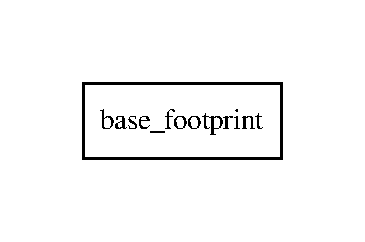
\includegraphics[width=70truemm, clip]{images/urdf_graph_only_base_footprint.pdf}
  \caption{URDF Tree (\textsf{base\_footprint} Only)}
  \label{fig:urdf_graph_only_base_footprint}
\end{figure}

\end{document}